\section{Digital Elevation Model Generation}
\label{sec:dem-generation}

\subsection{Purpose and evidential status}

No observed digital elevation model (DEM) was available for the study area.
The terrain used in this work was therefore generated as a deterministic
scenario surface rather than reconstructed from a topographic survey.  This
distinction is important: the elevations are stored as nominal metres above
mean sea level (AMSL), but the generation metadata states explicitly that they
are not tied to a surveyed vertical datum.  Consequently, the DEM supports
controlled numerical experiments and reproducibility tests; it does not
constitute evidence of the elevation at any particular location in Gurugram.

The generation pipeline used the reprojected domain polygon and land-use/land-
cover (LULC) roughness layer at
\path{data/interim/domain_epsg32643.gpkg} and
\path{data/interim/roughness_epsg32643.gpkg}, respectively.  Both inputs
were handled in EPSG:32643 (WGS~84/UTM zone~43N).  The configured raster cell
size was \(5.0\)~m.  The domain bounds recorded in the metadata were
686895.7867--714352.5363~m easting and
3135200.1244--3161045.8374~m northing.  Alignment of these bounds to the
configured cell size produced a 5170 by 5492 raster.  A cell-centre geometry
mask selected 17,284,848 valid domain cells; cells outside this mask were
excluded from the calculations and exported with a nodata value.

The input validation report contained no critical errors.  The mesh comprised
82,921 polygon elements in one connected component, with no invalid
geometries, degenerate triangles, or internal gaps reported.  Rainfall
validation likewise reported no missing timestamps or critical errors.  The
only validation warning was that the domain source was stored as a closed line
perimeter rather than as a polygon.  The DEM implementation handles this
representation by polygonising the closed perimeter in memory; it does not
alter the raw source geometry.

\subsection{Base terrain construction}

The base surface combined coherent multi-octave noise with a planar regional
gradient.  Coherent noise follows the construction introduced by
Perlin~\cite{Perlin1985}, but its use here was specifically parameterised for
this synthetic domain.  The implementation sampled two-dimensional noise on a
100.0~m control grid and resampled it cubically to the 5.0~m DEM grid.  The
noise scale was 2500.0~m, with five octaves, persistence 0.5, lacunarity 2.0,
and random seed 42.  Over the valid domain, the sampled noise was centred using
its minimum and maximum, scaled to the interval from \(-1\) to \(1\), and
clipped to that interval.  Its configured relief amplitude was 6.0~m about a
base elevation of 225.0~m.

A planar component imposed a total regional elevation difference of 8.0~m
along the valid-domain projection.  The configured downslope azimuth was
225.0 degrees clockwise from north, representing drainage towards the
south-west rather than an isotropic noise surface.  This direction is a
modelling assumption embedded in the configuration; it was not inferred from
surveyed elevations.  The fixed seed and the complete set of spatial and
spectral parameters are recorded in
\texttt{data/synthetic\_dem/metadata.json}, permitting exact regeneration of
the stochastic component.

\subsection{LULC-based urban conditioning}

The roughness layer provided broad LULC polygons but did not contain surveyed
road centre-lines or building footprints.  The conditioning step therefore
used LULC only as a proxy for urban microtopography.  The implementation
rasterised five normalised classes: Water, Built-up, Bare/Open, Low vegetation,
and Tree cover.  The metadata reports no unclassified cells within the domain.

Within Built-up polygons, a Euclidean distance transform separated boundary
cells from polygon interiors.  Built-up cells no farther than 10.0~m from a
class boundary were treated as road-corridor proxies and lowered by 0.15~m;
cells farther inside were treated as building-block proxies and raised by
0.60~m.  This procedure identified 1,054,580 road-proxy cells and 5,320,893
building-proxy cells.  Water cells were lowered by 0.35~m and Tree-cover cells
were raised by 0.05~m.  Bare/Open and Low-vegetation cells retained the base
surface.  These offsets are scenario assumptions, not measurements of kerb,
road, vegetation, or building heights.

Eight explicit waterlogging scenarios were then placed at seed-selected
locations within Built-up land.  Each feature was a circular bowl of 40.0~m
radius and 0.30~m maximum depth, with the lowering decreasing linearly to zero
at the perimeter.  The requested and created counts were both eight, and the
metadata records every centre coordinate together with the common radius and
depth.  Seed 42 was used for both the base terrain and depression placement.
The resulting LULC cell counts are reported in Table~\ref{tab:dem-lulc}.

\begin{table}[htbp]
    \centering
    \caption{Valid DEM cells assigned to each rasterised LULC class, as
    recorded in the generation metadata.}
    \label{tab:dem-lulc}
    \begin{tabular}{lr}
        \hline
        LULC class & Cell count \\
        \hline
        Water & 220,744 \\
        Built-up & 6,375,473 \\
        Bare/Open & 353,800 \\
        Low vegetation & 7,992,646 \\
        Tree cover & 2,342,185 \\
        \hline
        Total & 17,284,848 \\
        \hline
    \end{tabular}
\end{table}

\subsection{Hydrological conditioning}

Depression filling was implemented with PyFlwDir version 0.5.12 using the
Wang--Liu method~\cite{WangLiu2006}.  The metadata documents this backend as a
substitution for RichDEM 0.3.4 because the latter's NumPy requirement was
incompatible with the NumPy requirement of ANUGA 3.2 or later in the project
environment.

The configured policy was \texttt{selective}, with intentional-depression
preservation enabled and a fill tolerance of 0.0001~m.  The implementation
first computed a completely filled surface using edge outlets.  It then
restored the original elevations wherever the intentional-depression mask was
true.  Thus, algorithmically detected sinks outside the prescribed
waterlogging scenarios were removed, while the explicitly constructed
scenario depressions remained available to store water in subsequent
simulations.

The complete-fill diagnostic identified 4,838,632 cells that would be raised
by more than the tolerance, with a maximum required fill depth of
5.4481964~m.  After selective restoration, 649 cells still met the sink
criterion; all 649 were within the intentional-depression mask and the
reported number of unexpected remaining sink cells was zero.  These counts
establish consistency with the implemented classification rule.  They do not
demonstrate that depressions in the synthetic surface correspond to observed
waterlogging locations.

\subsection{Exported product and diagnostics}

The conditioned elevation was exported as a single-band, compressed
32-bit floating-point GeoTIFF at
\texttt{data/synthetic\_dem/dem.tif}.  The raster retains EPSG:32643 and the
5.0~m affine transform; invalid or out-of-domain cells use \(-9999.0\) as
nodata.  The generation metadata records a minimum elevation of
216.6333~m, a maximum of 233.4408~m, a mean of 225.2339~m, and a standard
deviation of 2.5799~m over the valid cells.  These values describe the
generated scenario and should not be interpreted as a validation against
observed terrain.

Figure~\ref{fig:dem-diagnostics} presents the generated hillshade, slope field,
and flow-accumulation diagnostic.  In the hydrological-conditioning module,
flow accumulation is derived from D8 routing with edge outlets and expressed
as upstream contributing area in raster cells.  The figure provides a visual
check of surface structure and drainage connectivity, rather than independent
validation of the synthetic elevations.

\begin{figure}[htbp]
    \centering
    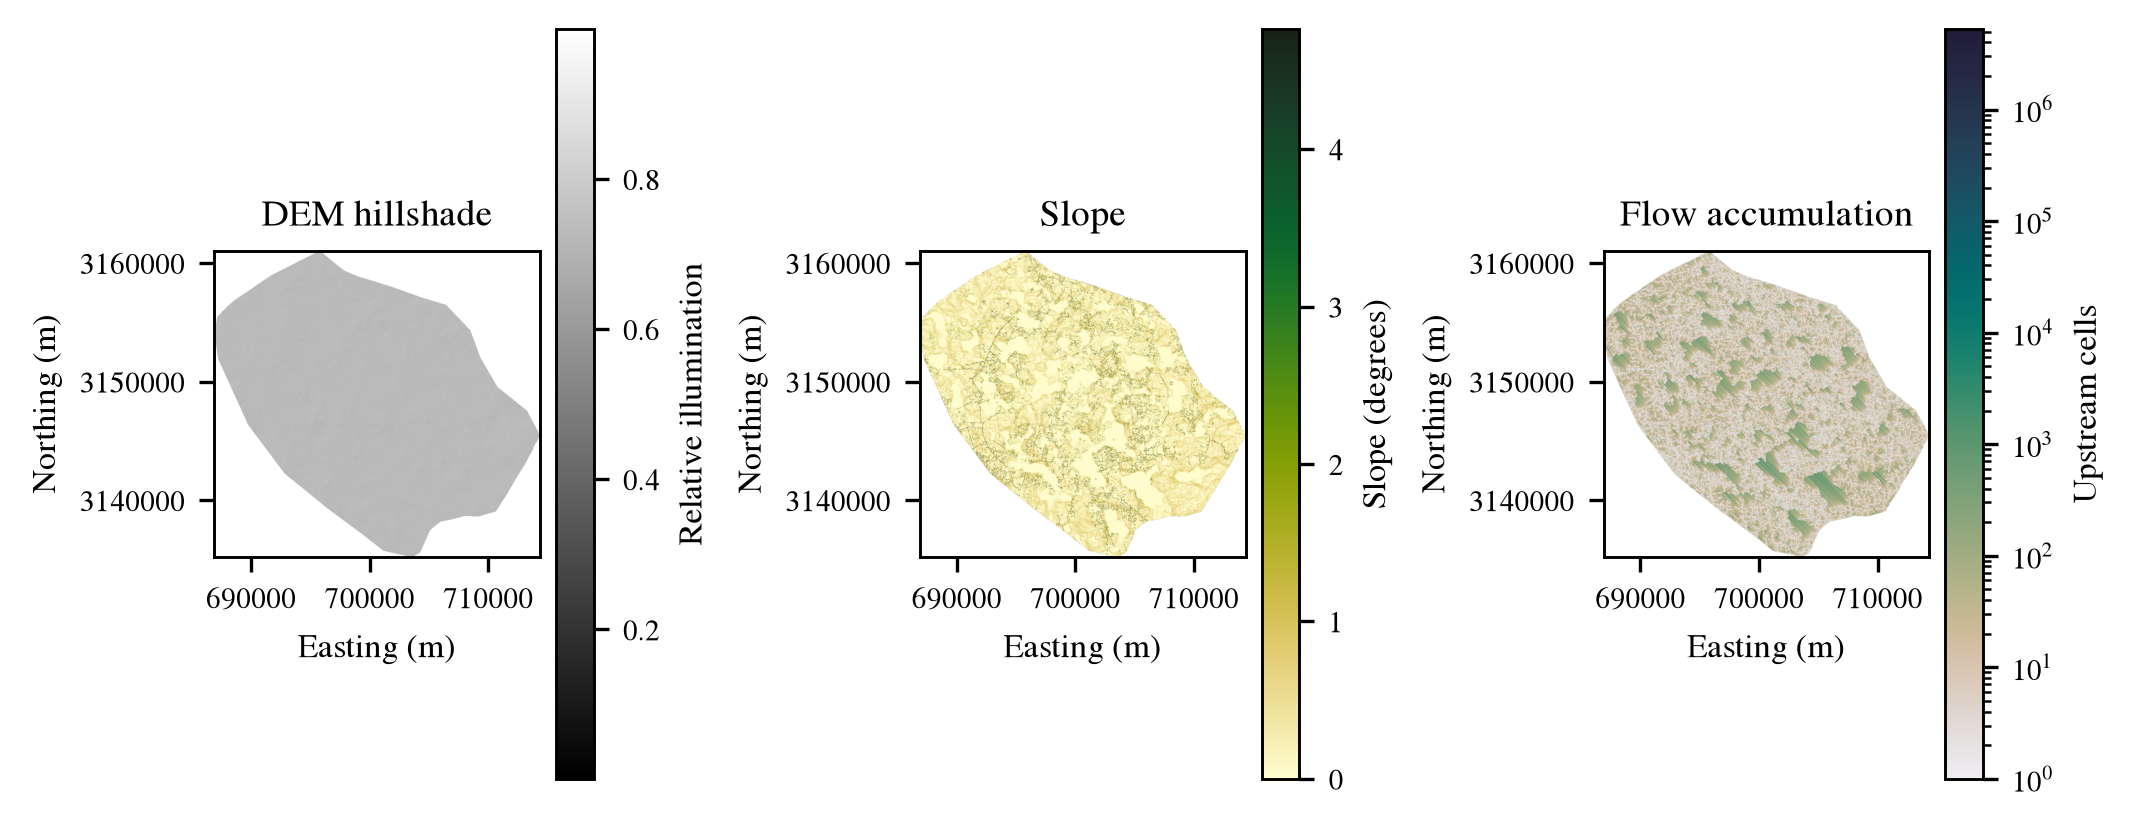
\includegraphics[width=\textwidth]{figures/dem_diagnostics.png}
    \caption{Diagnostics for the final synthetic DEM: hillshade (left), slope
    in degrees (centre), and D8 upstream contributing-cell accumulation
    (right).}
    \label{fig:dem-diagnostics}
\end{figure}

\subsection{Limitations}

The principal limitation is structural: broad LULC polygons and a prescribed
regional gradient cannot recover surveyed ground levels, drainage invert
levels, road crowns, kerbs, or individual building footprints.  In addition,
the eight preserved depressions encode controlled waterlogging scenarios
rather than observed sites.  The relatively large maximum complete-fill depth
also shows that hydrological conditioning materially altered parts of the
unconditioned synthetic surface.  Accordingly, later flood-model results
should be interpreted as comparisons of numerical and hybrid methods under a
reproducible synthetic terrain scenario.  Claims about real-world inundation
depths or locations would require an observed, vertically referenced DEM and
independent hydrological validation data.
